\documentclass[12pt]{article}
\usepackage{graphicx} % For including graphics
\usepackage{hyperref} % For URLs and hyperlinks
\usepackage{amsmath} % For math symbols
\usepackage{enumitem} % For customized lists
\usepackage{geometry} % For page margins
\usepackage{xcolor} % For colored text
\usepackage{titlesec} % For title formatting
\usepackage{fancyhdr} % For headers
\usepackage{setspace} % For spacing
\usepackage{graphicx}
\usepackage{multirow}
\usepackage{adjustbox} % For scaling the table
\usepackage{array} % For defining column widths and centering
\usepackage{geometry} % For margin adjustments
\usepackage{booktabs} % For better looking tables
\usepackage{caption}
\usepackage{subcaption}
\usepackage{float}
\usepackage{rotating}      % For sideways tables
\usepackage{tabularx}      % For automatically adjusting column widths
\usepackage{enumitem}      % For controlling list spacing
\usepackage{placeins}  % For \FloatBarrier
\usepackage{caption}
\usepackage{titlesec}  % Required for custom section titles
\usepackage{xcolor}

% Page setup
\geometry{a4paper, margin=0.75in} % Adjust margins to allow more space
\setlength{\parindent}{0pt} % Remove indentation
\captionsetup{font=scriptsize}  % Change 'small' to any size: footnotesize, scriptsize, etc.

\setcounter{tocdepth}{5}
\setcounter{secnumdepth}{5}
\newcommand{\paragraphs}[1]{\paragraph*{#1}\mbox{}\\}
\newcommand{\subparagraphs}[1]{\subparagraph*{#1}\mbox{}\\}

\renewcommand{\arraystretch}{1.2} % Adjusts the row height

% Title formatting with indentation for sections
% \titleformat{\section}{\bfseries\large\hspace*{1cm}}{\thesection.}{1em}{}
% \titleformat{\subsection}{\bfseries\hspace*{1cm}}{\thesubsection.}{1em}{}
% \titleformat{\subsubsection}{\bfseries\hspace*{2cm}}{\thesubsubsection.}{1em}{}

% Adjust paragraph indentation
\newenvironment{indentedsection}{
    \setlength{\parindent}{1cm} % Indent paragraphs
    \setlength{\leftskip}{1cm} % Indent entire section content
}{}

% Header setup
\pagestyle{fancy}
\fancyhf{}
\fancyhead[L]{Group No: C1}
\fancyhead[C]{ME 407 -- Fall 2024}
\fancyhead[R]{\thepage}

% Horizontal line
\renewcommand{\headrulewidth}{0.4pt}


% Begin Document
\begin{document}

% Main title and keyword section
\begin{center}
    \vspace{1em} % Add some space
    \textbf{\LARGE PROJECT PLANNING and MANAGEMENT \\
    \vspace{8pt}REPORT}\\
\end{center}

% Start of sections

\section*{I. Introduction}
This report presents the planning and organization for the management of the Table Tennis Ball Pitcher Machine project. A structured timetable is established to guide each project phase, from problem definition to testing, ensuring efficient workflow. This document details the planning approach, task distribution and timeline established to ensure systematic project execution. The project members responsible for the tasks are abbreviated as in Table \ref{tab:teammembere}.

\begin{table}[h!]
\centering
\begin{minipage}{0.45\textwidth}
    \centering
    \begin{tabular}{|c|c|}
    \hline
    \textbf{Name} & \textbf{Abbreviation}\\
    \hline
    Abdullah Can Seyhanlı &  ACS\\
    Altay Ata Ateş & AAA\\
    Arman Utku Aydın & AUA\\
    Abdullah Salih Taşdelen &  AST\\
    \hline
    \end{tabular}

\end{minipage}%
\hfill
\begin{minipage}{0.45\textwidth}
    \centering
    \begin{tabular}{|c|c|}
    \hline
    \textbf{Name} & \textbf{Abbreviation} \\
    \hline
    Bilal Açıksöz & BA\\
    Kutay Can Yapıcı & KCY\\
    Ömer Aslan & ÖA\\
    Özge Dilan Tuna & ÖDT\\
    Yunus Emre Özçelik & YEÖ\\
    \hline
    \end{tabular}    
\end{minipage}
    \caption{The Members of the Project}
    \label{tab:teammembere}
\end{table}

    
\section*{II. Organization of the Project}

In this section of the report, the definition of tasks and the workload distribution among the team members are presented. As a first step, a literature survey is conducted to define the problem. After defining the problem project requirements and specifications are determined. In consideration of these steps, the functions of the project are decomposed. \\

\subsection*{II.A Explanation of the Tasks and Their Definitions}

\subsubsection*{1. Literature Survey}
At the start of a project, literature survey carries great importance so as to gather information about the related products and technologies available on the market. Also, research regarding the patents related to the project is conducted. Ultimately, the literature survey gives insight about the direction the project will take. 

\paragraphs{1.a. Commercial Product Research (AAA, AUA, BA)}
This section involves the research of the products on the market. Prices of these products, their design criteria and to what extent they satisfy the said criteria are evaluated. Studying the interest on the market regarding the field and products also contributes to the project. 

\paragraphs{1.b. State of the Art Research on Related Projects (ÖDT, AST, KCY)}
In this part, scientific papers and technological advancements that are related to the project are researched. State of the art research, unlike the commercial product part, takes into consideration the technologies that are new and some cutting-edge, thereby allowing for more creative ideas and open-minded thinking. 

\paragraphs{1.c. Patent Research (ACS, YEÖ, ÖA)}
Patent research is a very crucial step in a design process. A product created without researching and knowing the patented products related to the project beforehand is not viable. The components and the products similar to the design in mind must be determined.  

\subsubsection*{2. Project Initiation}
The project needs to be initialized and worked over after the literature survey is completed. An investigation process should be completed by using a step-by-step approach. After all the steps are completed, the project is to be completely initiated.

\paragraphs{2.a Problem Definition (AAA, YEÖ)}
A problem needs to be defined properly if a design is to be made as a solution. Determining the problem correctly and thoroughly is important and makes it easier to create a good design in the later stages of the process.

\paragraphs{2.b Project Requirements (ÖDT, KCY, ÖA)}
 In this step the requirements that should be met and the functions the product must be able to perform are defined without giving the numerical constraints or any measurable limitations. 

\paragraphs{2.c Design Specifications (BA, AUA)}
The requirements specified on the previous step are defined numerically in this step. Functions the product must be able to perform and the restrictions it is subjected to are indicated in a quantitative way.  

\paragraphs{2.d Design Criteria (ACS, AST)}
In this step, the design criteria for the product should be stated, and the percent weight of importance for each of the criteria are assigned. 

\subsubsection*{3. Functional Decomposition}
Functional decomposition is a process to separate an engineering solution/device into its subfunctions. It is created based on need statements which is the process of converting customer needs into solution neutral engineering actions. Each subfunction should be suitable for individual examination. After the functional decomposition is performed, each function is investigated to find suitable solutions. 

\paragraphs{3.a. Flow Chart (YEÖ, BA)}
Flow chart is a type of functional chart which includes all the subfunctions from the main function to the subfunction in a logical or temporal order with material, information, and energy inputs. These subfunctions are grouped by considering a common function to be performed. For the given inputs the outputs are also determined, considering the conservation.  

\paragraphs{3.b. Function Tree Chart (YEÖ, AST, AAA)}
Functional tree chat is another type of functional decomposition. Main difference from the flow chart is that function tree is designed with levels starting from the main function extending with relevant subfunctions till the solution of each subfunction. 

\subsubsection*{4. Project Planning }
It is crucial to plan the schedule the project properly. Insufficient planning may lead to many problems, such as production errors and delays of the reports. To be able to plan properly, it is important to know the members of the group well and assign them tasks according to their interests and knowledge areas. 

\paragraphs{4.a. Project Organization (ALL TEAM)}
Project Organization as a task involves setting up the structure, roles, and processes necessary for a project to run efficiently and achieve its objectives. Project Organization is foundational to project success, as it sets up the necessary framework, team alignment, and resources to achieve project goals. 

\paragraphs{4.b. Task Explanation and Assignment (AUA)}
At the start of a project, first step is to determine the tasks. The task definitions must be done clearly and in a way that fully encompasses what the task should achieve. So, it is easier to determine how to approach each task, and it is possible to assign them to the member that is most capable of undertaking it. 

\paragraphs{4.c. Timetable and Timeline Creation (AUA, AST)}
Aside from assigning the tasks and setting their definitions, it is important to allocate the time to complete these tasks. To achieve it, a timetable should be constructed and it has to be ensured that it is followed properly. For the timeline, it is necessary to fill a Gantt chart with the durations decided at the timetable, including the specific dates. 

\subsubsection*{5. Conceptual Design}
Conceptual design is mainly composed of two steps: concept generation and concept evaluation. 

\paragraphs{5.a. Morphological Chart (ALL TEAM)}
Morphological chart is a chart where generated concepts that are considered to be logical solutions at first look are listed. It is a method for concept generation. This process is done for each sub-function obtained during the functional decomposition and listed in the morphological chart. Generated concepts are illustrated with sketches which are in conceptual level, not necessarily in the engineering level. All the concepts must be in the same level and should perform the function for sure.

\paragraphs{5.b. Concept Evaluation (ALL TEAM)}
At this step, the generated concepts which are listed in morphological chart are evaluated considering each engineering criteria, choosing from several types of evaluation methods. The concepts are then graded. The results obtained from this step determines the optimal solution/s for each sub-function.

\subsubsection*{6. Detailed Design}
At this step, the process which have been theoretical up to this point and the generated concepts take its final shape and the product architecture is determined. All the design parameters are quantified and parts that will perform the functions take form. This step is highly iterative and requires good communication among the team.

\paragraphs{6.a. Kinematic Design (YEÖ, ACS)}
This process includes kinematic analysis, synthesis, and optimization for all parts and parameters of the system. It requires hand calculations and geometry-based software.
\paragraphs{6.b. Static Analysis (YEÖ, AAA)}
 This process includes structural analysis which includes material selection and stress analysis of the parts. It requires hand calculations and engineering software. 
 
\paragraphs{6.c. Geometric Analysis (AUA, BA)} 
This process includes CAD modeling, and geometrical parameter determination. 
\paragraphs{6.d. Circuit Design (AST)}
In this process the circuitry needed for the motor control, buttons, encoders etc. and also the voltage regulators will be designed. It is crucial for not harming any electrical/mechanical components.


\subsubsection*{7. Manufacturing}
\paragraphs{7.a. Procurement (AUA, AST)}
After the analyses are complete, the materials chosen according to the market research conducted previously are to be supplied. Procuring the materials is a crucial part since manufacturing process cannot start without deciding on and obtaining the materials needed. 

\paragraphs{7.b. Determination of Manufacturing Methods (YEÖ, KCY)}
Regarding the project requirements, design specifications and the materials, the suitable methods to manufacture the system are to be decided on. In this part, the priority is to provide the sustainability of the material life and to avoid possible excessive expenses.   

\paragraphs{7.c. Producing the Parts (AAA, ÖA, BA)}
The necessary parts are to be produced by applying the manufacturing methods determined at the previous part.   
 
\paragraphs{7.d. Assembly (ACS, ÖDT)}
In the assembly section, the produced parts are to be joined together to create the final product. 

\paragraphs{7.e. Quality Control (AST, AUA)}

Quality control should be performed for each part produced to ensure the quality of the materials, make sure the standards are met, foresee the potential unexpected changes and deviations to avoid them as much as possible, and to increase the efficiency of the process. After the assembly is done, it is important to do a final quality control to obtain an overall result. 

\subsubsection*{8. Documentation}

\paragraphs{8.a Reports (ALL TEAM)}
From the beginning of the project, reports are to be written to record the project design procedure and explain the steps better. This part also makes it easier to plan the timeline and organize the time until the deadline. 

\paragraphs{8.b Drawings (KCY, YEÖ, AUA)}
It is important to have the drawings of each part of the system, which includes the tolerances, dimensions and constraints, in order to manufacture the parts designed. 

\paragraphs{8.c Calculations (AST, ACS, ÖA)}
The pre-design calculations should be included for speed, motion, power, space required and trajectory motion etc. to demonstrate that the solutions are viable for the project requirements. 

% Repeat for each task (e.g., Detailed Design, Manufacturing, Documentation)

\subsection*{II.B Time Table}

\begin{table}[h!]
\centering
\begin{minipage}{0.45\textwidth}
    \centering
    \scriptsize
    \begin{tabular}{|c|c|c|}
    \hline
    \textbf{Task ID} & \textbf{Duration} & \textbf{Team Members} \\
    \hline
    1.a & 2 weeks & AAA, AUA, BA \\
    1.b & 2 weeks & ÖDT, AST, KCY \\
    1.c & 2 weeks & ACS, ÖA, YEÖ \\
    2.a & 1 week & AAA, YEÖ \\
    2.b & 1 week & ÖDT, KCY, ÖA \\
    2.c & 1 week & BA, AUA \\
    2.d & 1 week & ACS, AST \\
    3.a & 1 week & YEÖ, BA \\
    3.b & 2 weeks & YEÖ, AST, AAA \\
    4.a & 1 week & ALL TEAM \\
    4.b & 1 week & AUA \\
    4.c & 1 week & AUA, AST \\
    5.a & 2 weeks & ALL TEAM \\
    \hline
    \end{tabular}
\end{minipage}%
\hfill
\begin{minipage}{0.45\textwidth}
    \centering
    \scriptsize
    \begin{tabular}{|c|c|c|}
    \hline
    \textbf{Task ID} & \textbf{Duration} & \textbf{Team Members} \\
    \hline
    5.b & 1 week & ALL TEAM \\
    6.a & 2 weeks & YEÖ, ACS \\
    6.b & 2 weeks & YEÖ, AAA \\
    6.c & 2 weeks & AUA, BA \\
    6.d & 1 week & AST \\
    7.a & 2 weeks & AUA, AST \\
    7.b & 1 week & YEÖ, KCY \\
    7.c & 3 weeks & AAA, ÖA, BA \\
    7.d & 1 week & ACS, ÖDT \\
    7.e & 1 week & AST, AUA \\
    8.a & 6 weeks & ALL TEAM \\
    8.b & 2 weeks & KCY, YEÖ, AUA \\
    8.c & 2 weeks & AST, ACS, ÖA \\
    \hline
    \end{tabular}
\end{minipage}
    \caption{Time table showing workload distribution}
\end{table}

\subsection*{II.C Timeline}
The Gannt Chart is in Appendix, Fig. \ref{fig:gannt}.

\section*{III. Summary and Conclusion}
In this report, planning and organization of the project is documented. It is of upmost importance that the fundamentals of the project is laid out clearly so as to ensure the project proceeds smoothly and with minimal obstacles, so the initial research and concept design parts are crucial. Accumulation of ideas and different concepts allow for a wide range of solutions to possible problems or discrepancies that might arise during the process. Another important step is to manage the team members and their tasks. For an effective and efficient project process, the communication and concord between team members, as well as assigning their undertakings according to their individual capabilities and strength is very important.
For the evaluation and conceptual design steps, software like Microsoft Excel are to be used for the organization of the criteria and concepts. For the detailed design further into the project, CAD software will be useful for the technical drawings, and the analysis parts will be carried out using analysis software tools. For the manufacturing part, CAM software is helpful to determine the methods of manufacturing, which will then be performed in machine shops, using various tools and methods depending on the part and material, such as additive manufacturing, turning/milling and even CNC machining.

% Prevent floats from passing this point
\FloatBarrier

% % References section
% \bibliographystyle{IEEEtran} % or any style you prefer
% \bibliography{bibliography}

% Yatay mi yapsak??
\begin{figure}
    \centering
    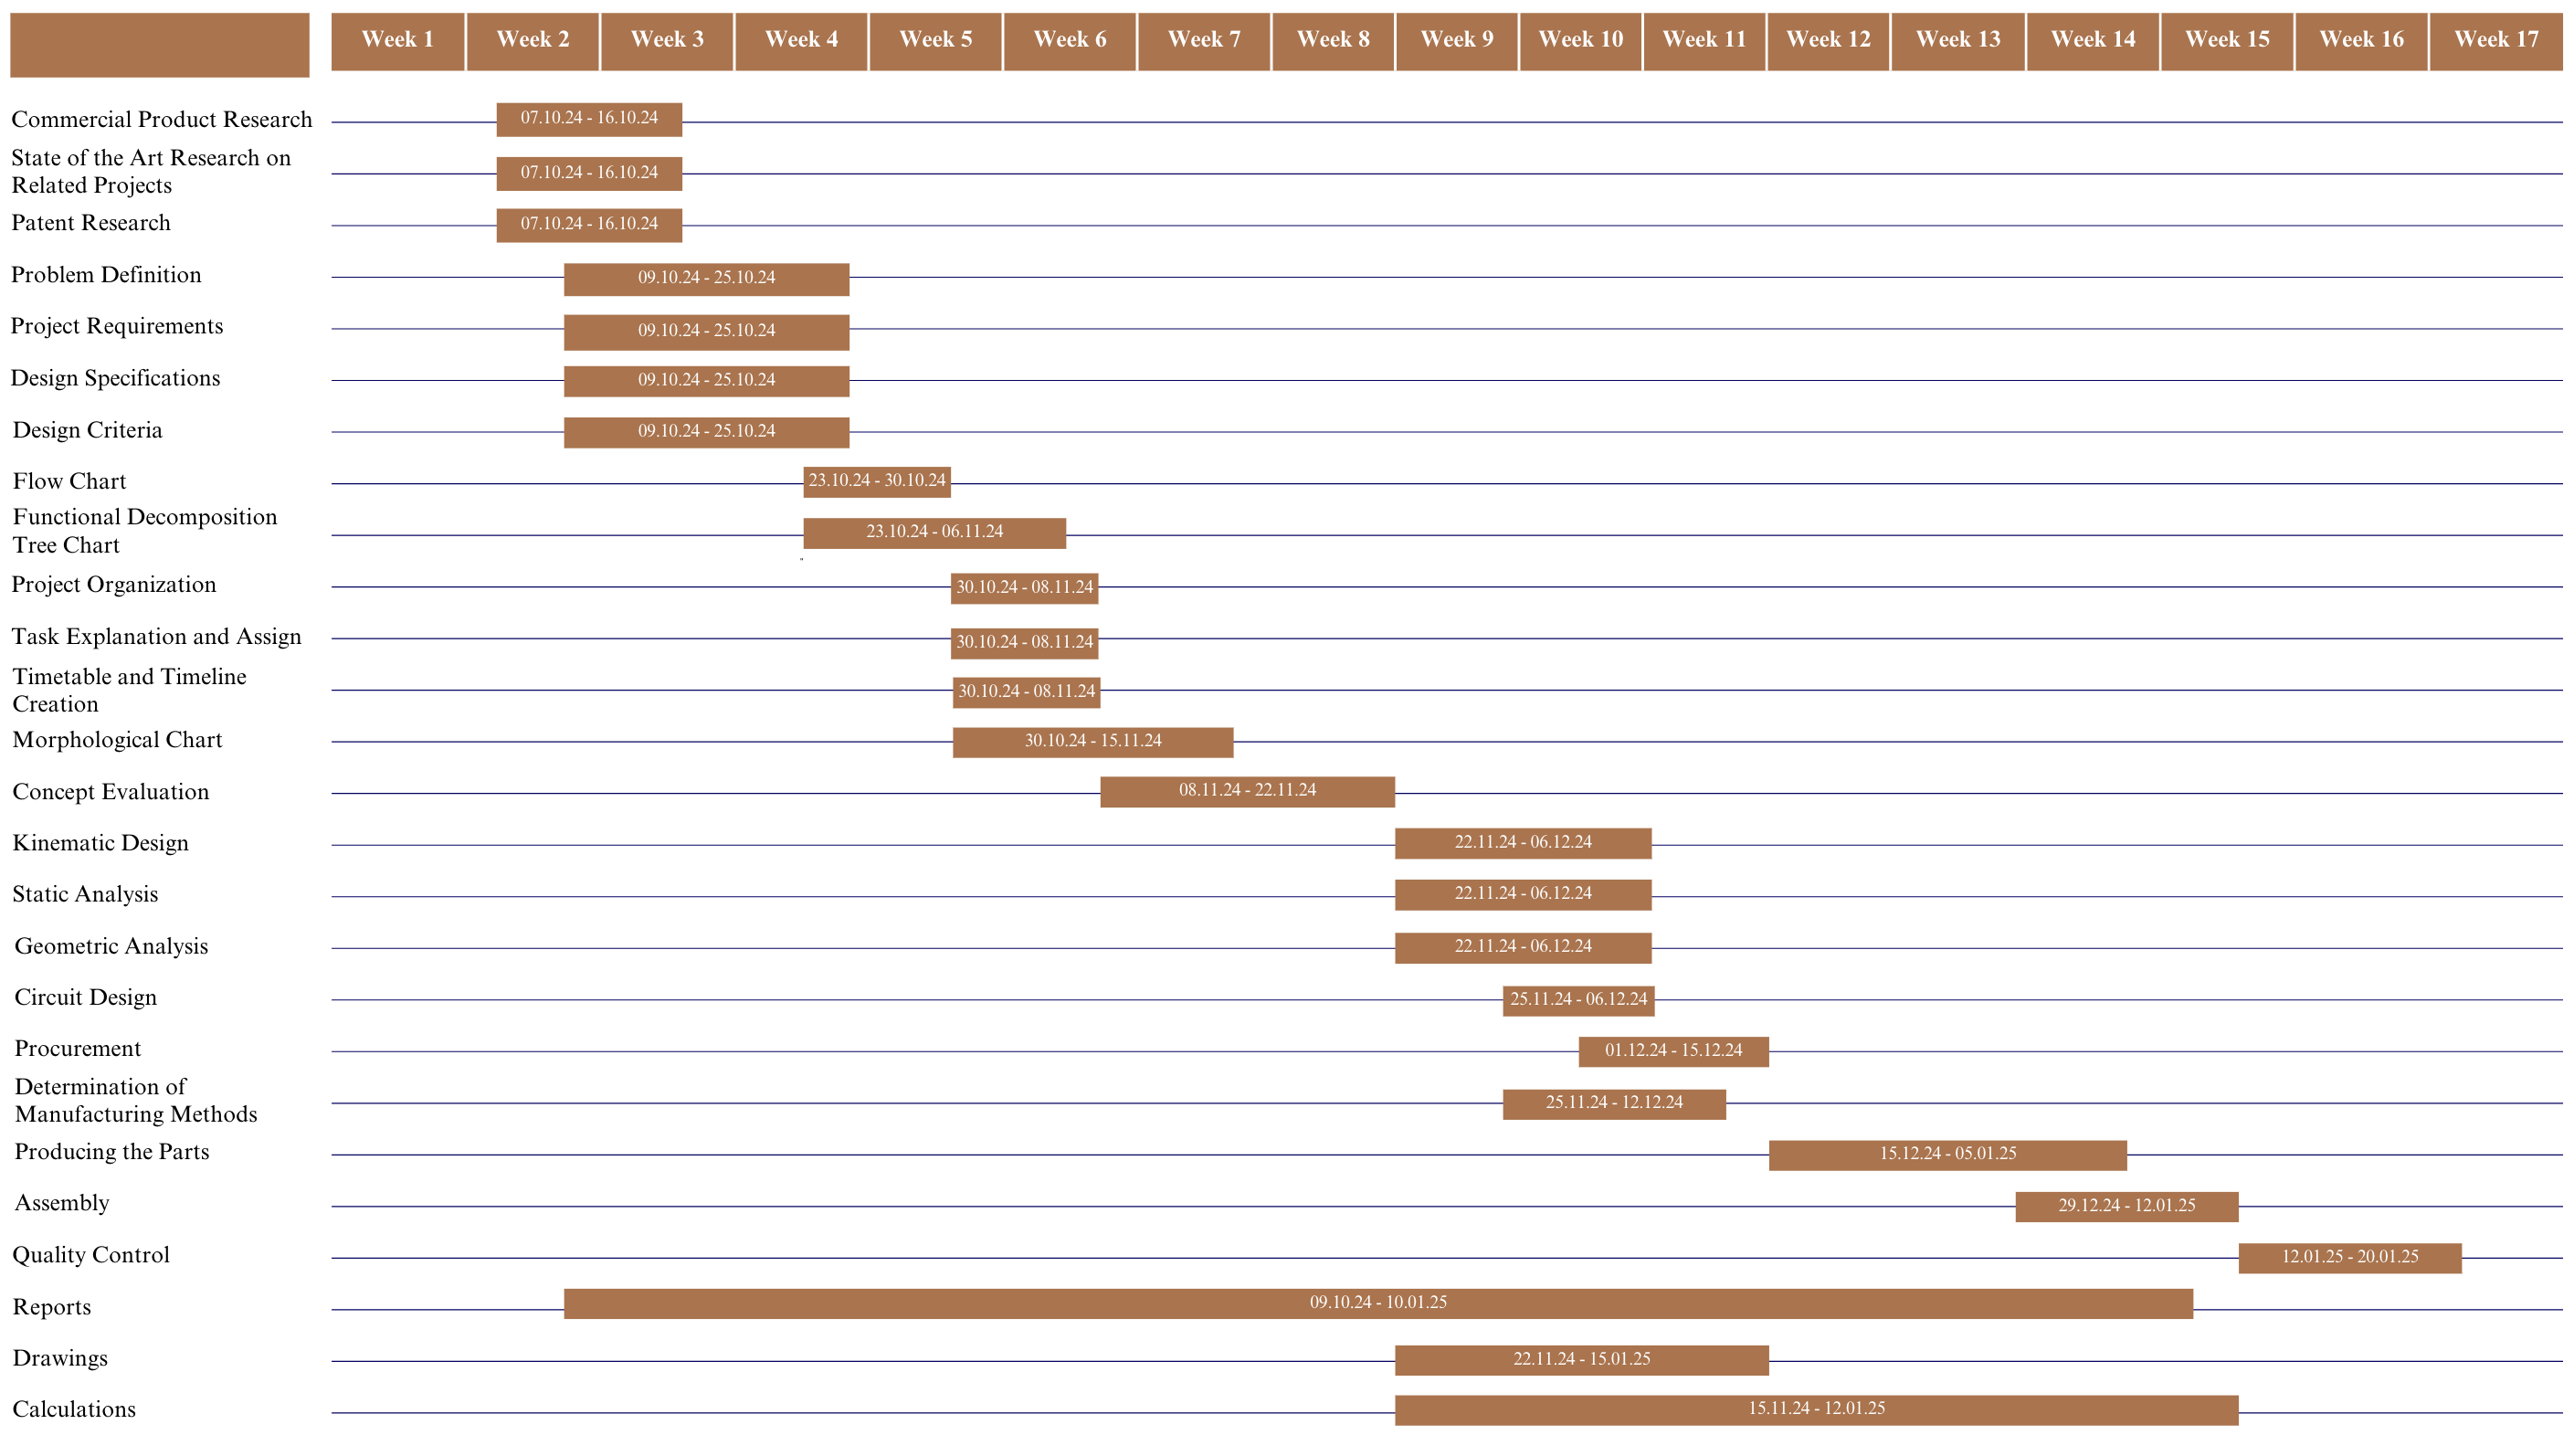
\includegraphics[angle=90, width=\linewidth, height=1.5\linewidth]{Ekran Resmi 2024-11-15 20.07.48.png}
    \caption{Gannt Chart}
    \label{fig:gannt}
\end{figure}

\end{document}

